\subsection*{Analysis Outliers Packages: Decreasing Trend}
\label{sec:analysisHexDecreasing}

\begin{figure}[htbp]
    \centering
    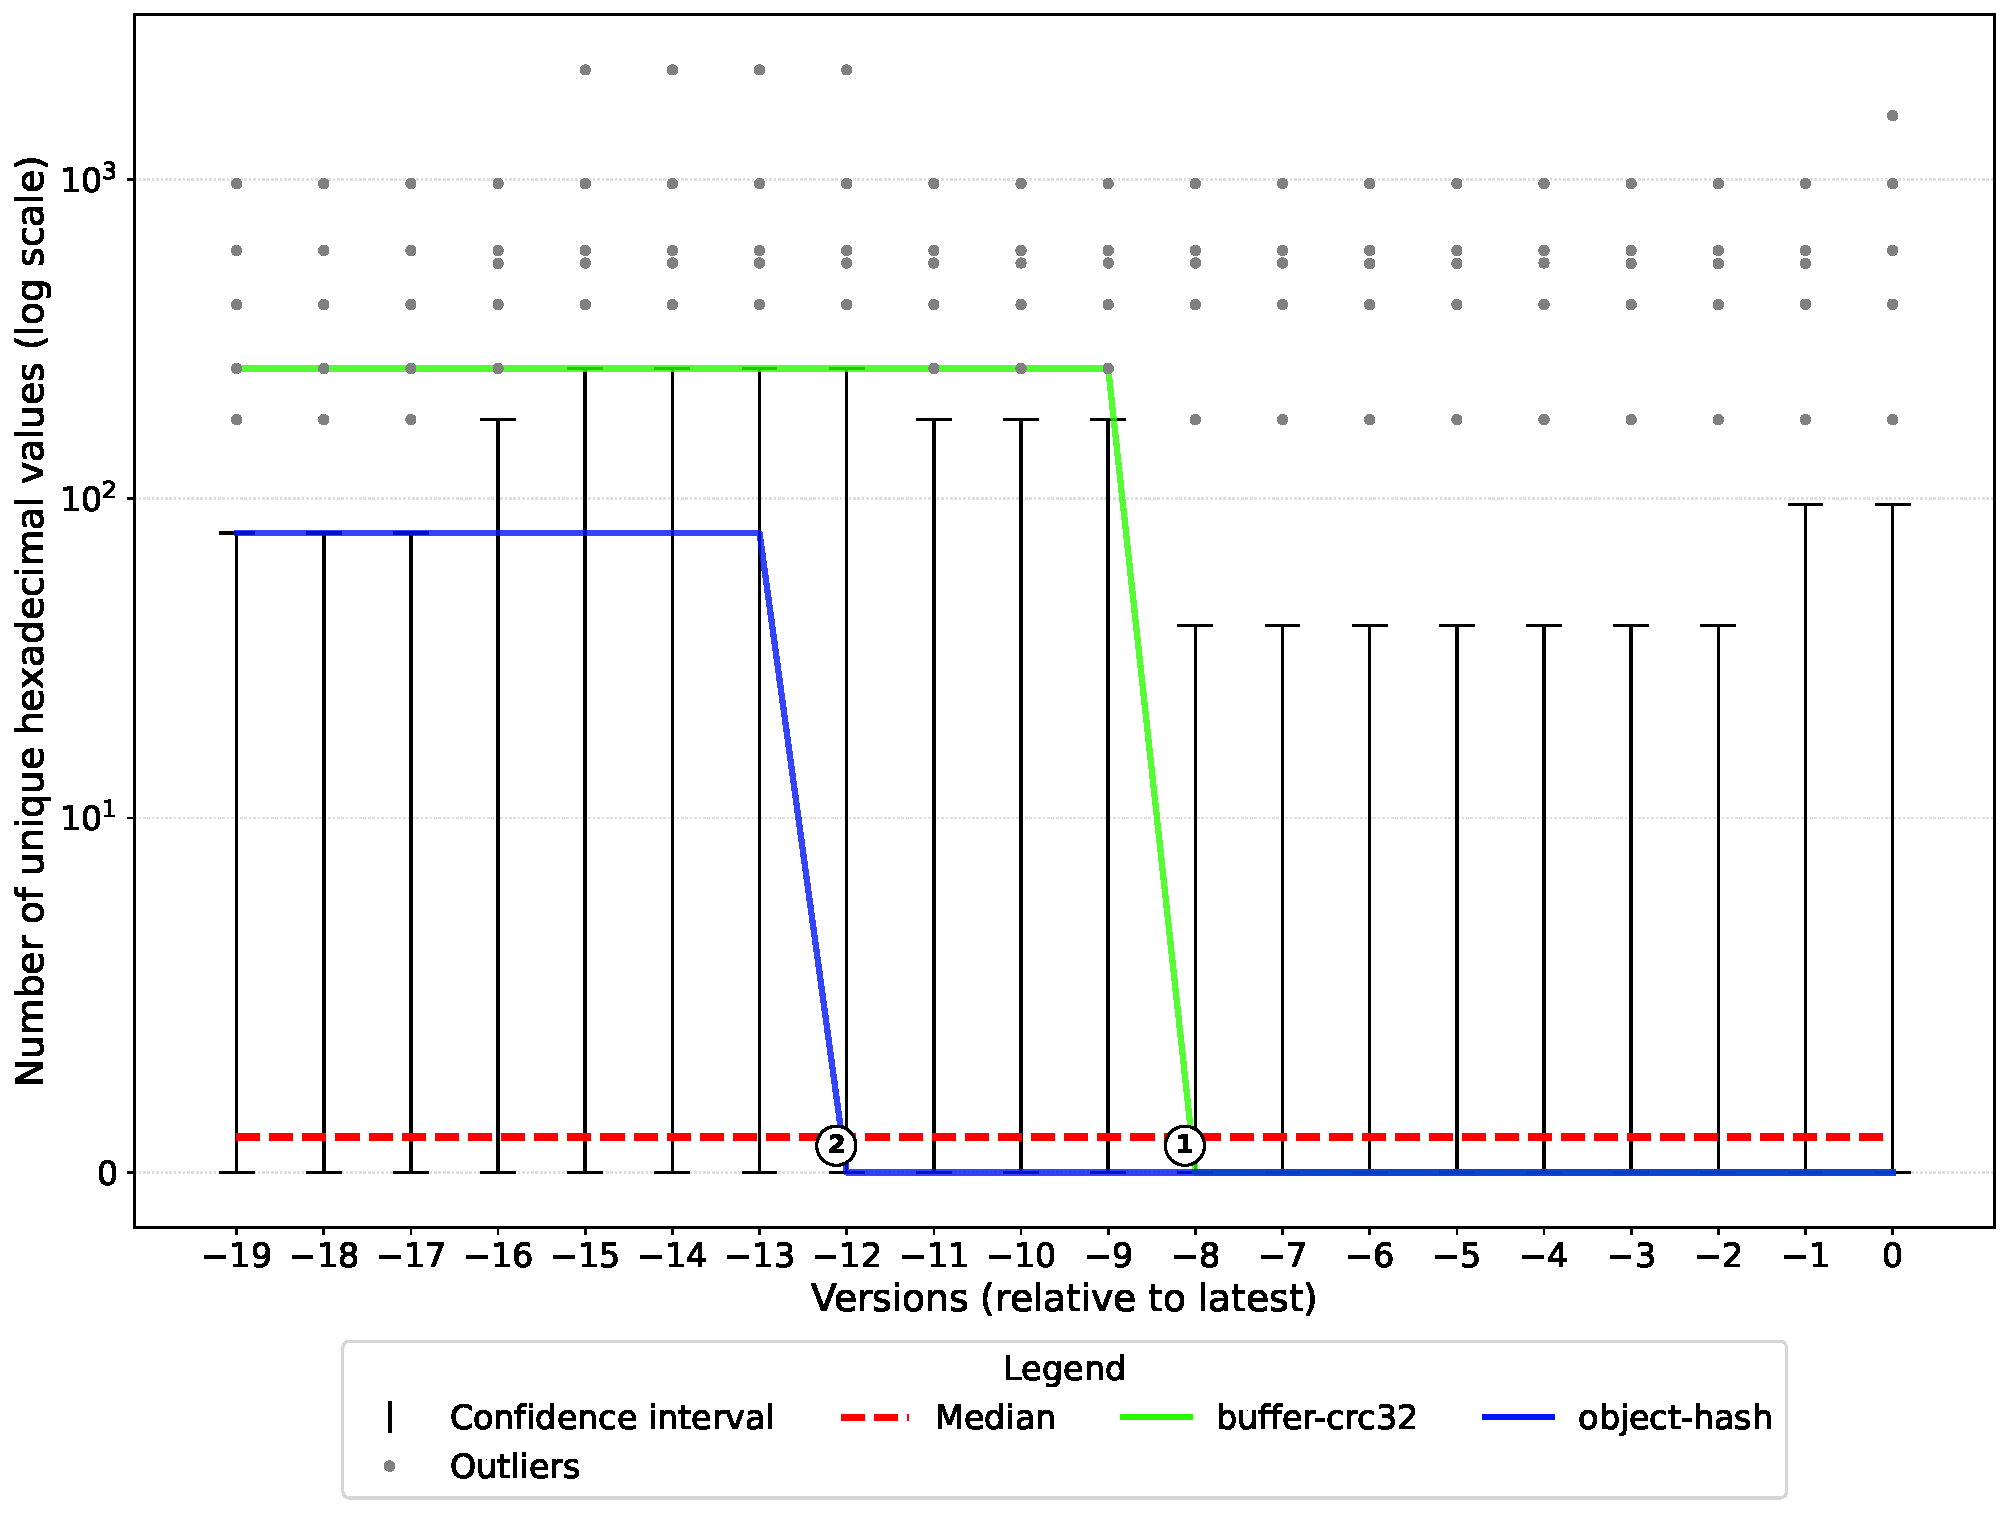
\includegraphics[width=\textwidth]{metrics/hex/hex_plot1_Decreasing_Trend.pdf}
    \caption{Outliers package Decreasing Trend for the Unique Hexadecimal Values Metric in Goodware dataset.}
    \label{fig:fig1HexDecreasing}
\end{figure}

The packages that had a considerable decrease from one version to the next are: \texttt{buffer-\\crc32} and \texttt{object-hash}.

\begin{itemize}
     \item \textbf{buffer-crc32:} The \texttt{buffer-crc32} package implements the \ac{CRC32} algorithm, 
    primarily used to detect accidental errors in data transmission or storage~\cite{buffer-crc32}.
    It is represented by the solid green line in \cref{fig:fig1HexDecreasing}.

    To make the data integrity check fast and efficient, the algorithm uses a CRC table, 
    a matrix of 256 pre-calculated values that prevents the processor from performing complex mathematical calculations 
    on every single byte.
    Specifically, until version 0.2.13 (the version before point 1 in \cref{fig:fig1HexDecreasing}), 
    the package stored these CRC table values in hexadecimal format.

    As shown at point 1 in \cref{fig:fig1HexDecreasing}, starting from version 1.0.0-RC1, 
    the developers optimized the package space by including in the tarball 
    the CRC table file generated using automatic build tools, such as minifiers.
    In this automated process, these build tools choose to convert the hexadecimal values into decimal format because it is more compact.
    While the mathematical value of the constants remained unchanged, 
    the number of unique hexadecimal values dropped from 256 to 0.


    \item \textbf{object-hash:} The \texttt{object-hash} package generates a hash from JavaScript objects and values~\cite{object-hash}.
    In \cref{fig:fig1HexDecreasing} (solid blue line), it can be observed that from version -19 to -17 (1.1.0 to 1.1.2),
    the package represented the upper limit of the confidence intervals for those versions, having 78 unique hexadecimal values.
    These values were all located in a test file, \texttt{object\_hash\_test.js}, which contained various tests to verify the package's correct operation.

    As shown at point 2 in \cref{fig:fig1HexDecreasing}, starting from version 1.1.7,
    the developers optimized the package space by excluding the test file from the tarball,
    as it is not essential for its functionality.
    The removal of this file caused the number of unique hexadecimal values to drop from 78 to 0.

\end{itemize}


\subsection*{Analysis Outliers Packages: Stable Trend}
\label{sec:analysisHexStable}

\begin{figure}[htbp]
    \centering
    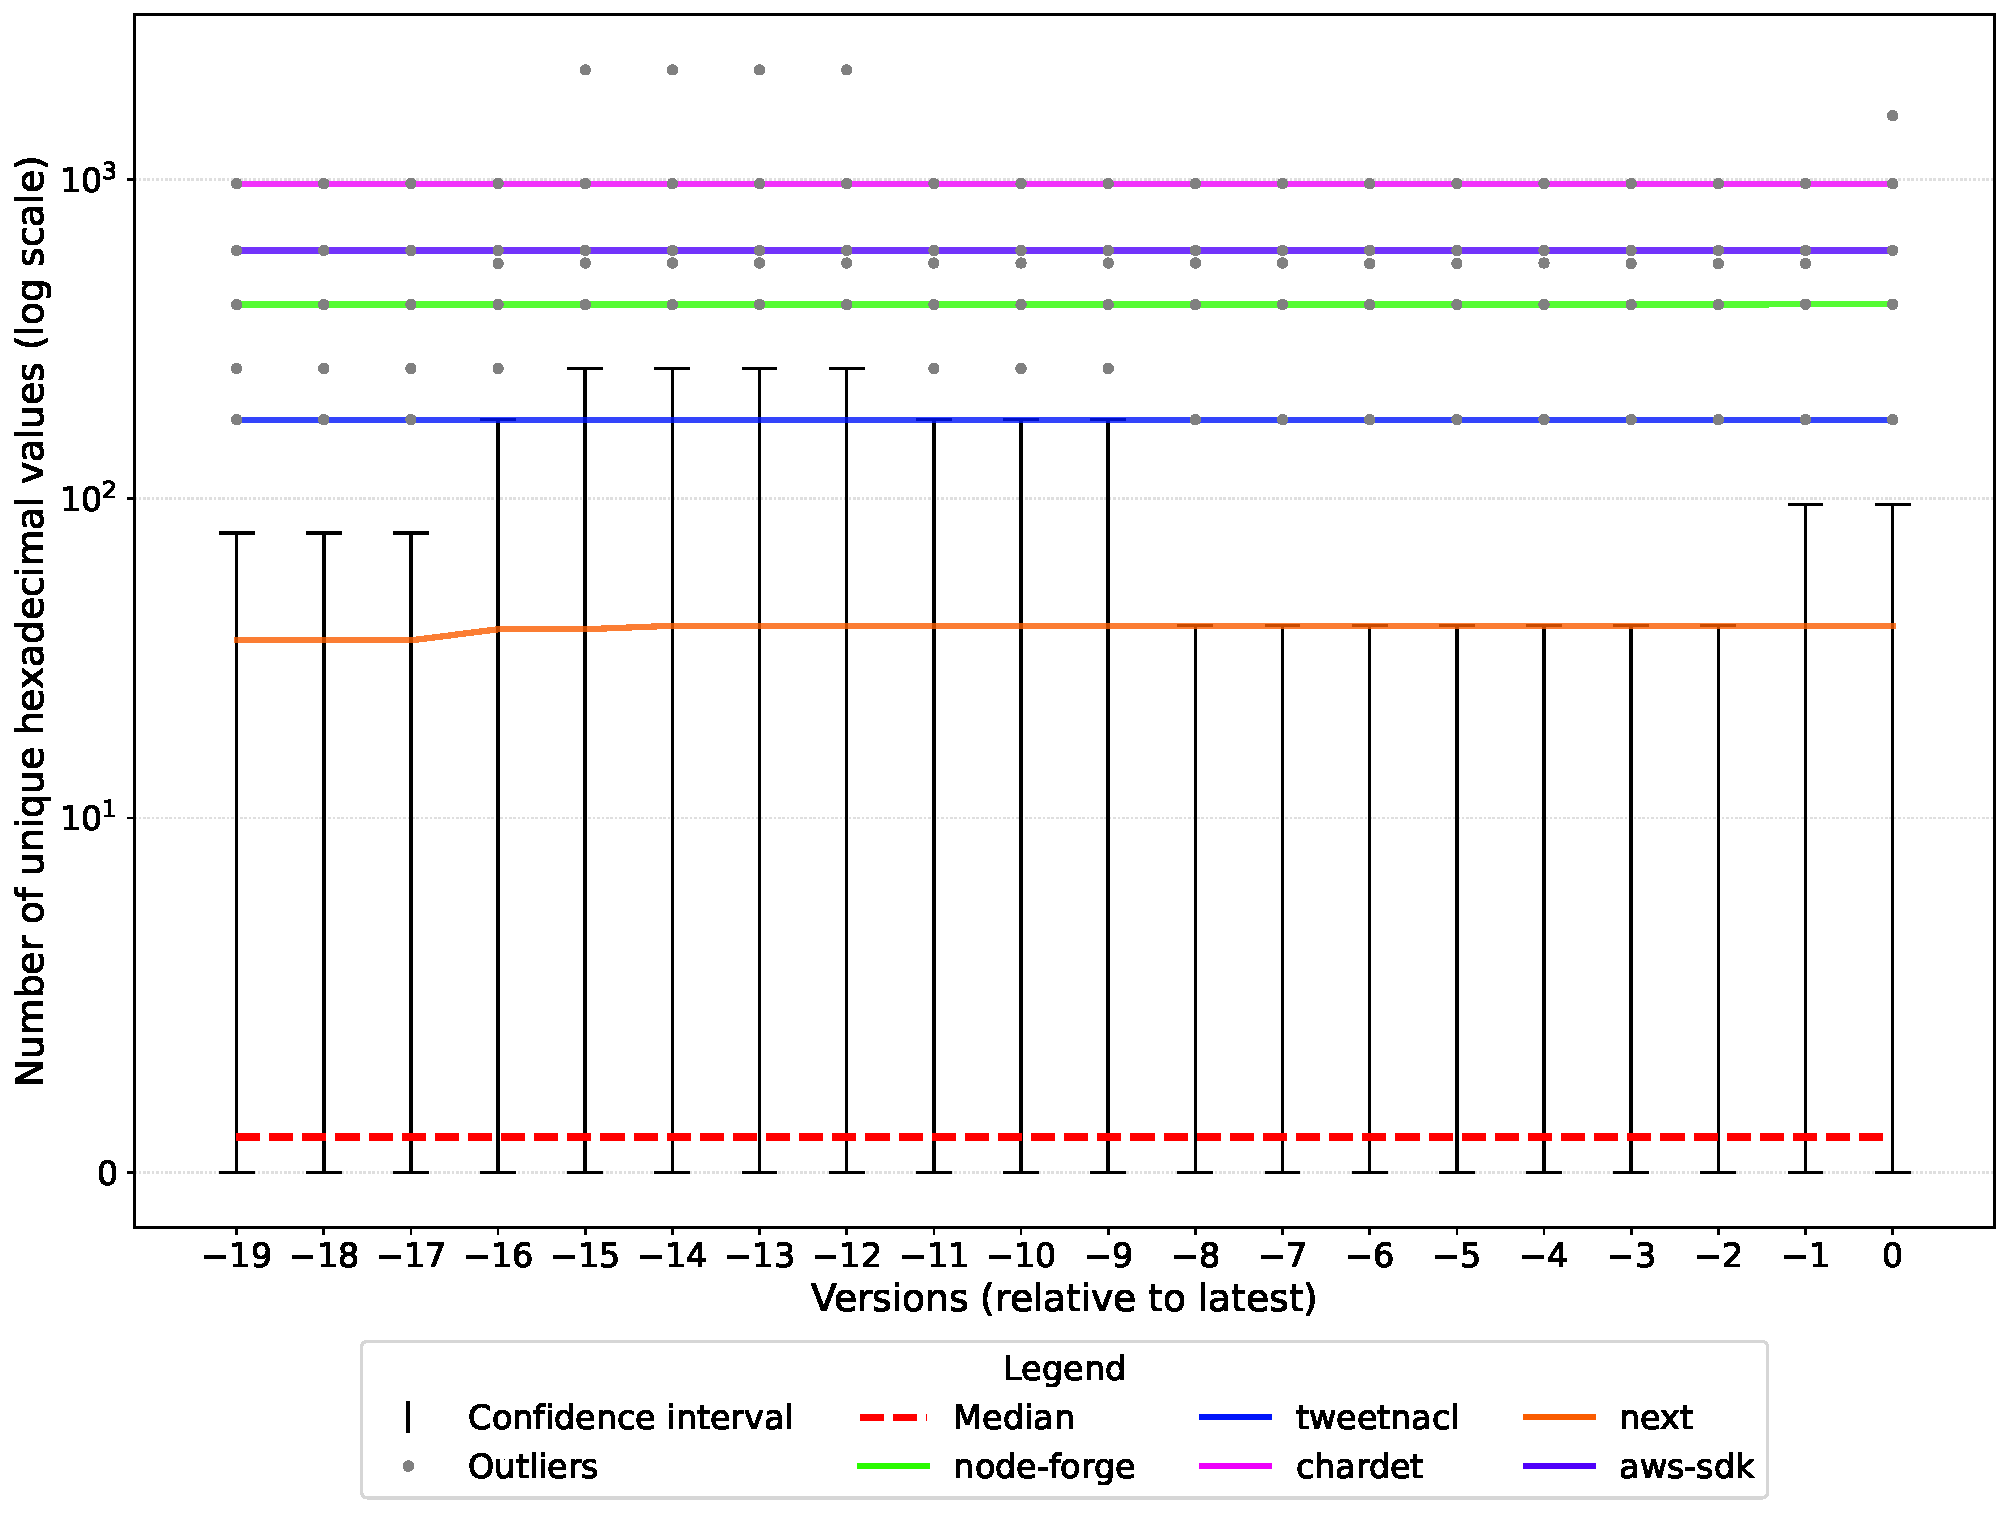
\includegraphics[width=\textwidth]{metrics/hex/hex_plot1_Stable_Trend.pdf}
    \caption{Outliers package Stable Trend for the Unique Hexadecimal Values Metric in Goodware dataset.}
    \label{fig:fig1HexStable}
\end{figure}

The remaining 5 highlighted packages had outlier values or values representing the upper limit of the confidence intervals
that remained constant across all 20 versions, without significant increases or decreases.
The packages exhibiting this trend are: \texttt{node-forge}, \texttt{tweetnacl}, \texttt{chardet}, \texttt{next}, and \texttt{aws-sdk}.

    \begin{itemize}
        \item \textbf{node-forge and tweetnacl:} Both packages are related to cryptography~\cite{node-forge, tweetnacl} and
        implement cryptographic primitives that use hexadecimal constants for their internal functioning,
        like \texttt{crypto-js} seen in \cref{sec:analysisHexIncreasing}.

        In \cref{fig:fig1HexStable}, \texttt{node-forge} (solid green line) has 406 unique hexadecimal values, 
        representing an outlier across all versions;
        while \texttt{tweetnacl} (solid blue line) has 177 unique hexadecimal values, representing the upper limit 
        of the confidence intervals for versions -16 and from -11 to -9, and representing an outlier for the remaining versions.

        \item \textbf{chardet:} This package detects character encoding, and uses 
        tables and byte maps in the form of hexadecimal constants,
        primarily located in the file \texttt{/lib/encoding/\\sbcs.js}~\cite{chardet}.

        Represented in \cref{fig:fig1HexStable} by the solid pink line,
        the package assumes 972 unique hexadecimal values, representing the most extreme 
        outlier for most versions. It was surpassed only by the \texttt{polished} package from version -15 to version -12, 
        and in the latest version (0) by the \texttt{crypto-js} package.

        \item \textbf{next and aws-sdk:} Finally, the \texttt{next} and \texttt{aws-sdk} packages contain 
        numerous JavaScript files in their tarballs that are
        generated by build tools and containing hexadecimal values.
        This behavior is the same as seen for the \texttt{polished} in \cref{sec:analysisHexIncreasing}
        and \texttt{buffer-crc32} packages in \cref{sec:analysisHexDecreasing}.

        In detail: the \texttt{next} package, a React full-stack framework~\cite{next} represented by 
        the solid orange line in \cref{fig:fig1HexStable}, has 40 unique hexadecimal values
        consistently across all versions, representing the upper limit of the confidence intervals for versions from -8 to -2.
        Conversely, \texttt{aws-sdk}, the official package for interacting with \ac{AWS} cloud services~\cite{aws-sdk} represented by 
        the solid purple line, has 600 unique hexadecimal values
        consistently across all versions, representing an outlier for all versions.

    \end{itemize}



\subsection{Comparison with Malware Dataset}
\label{sec:analysisHexComparisonMalware}

We analyzed when this metric is effective for detecting these four attacks (described in \cref{ch:AnalysisRecentAttacks}) and when it is not indicative.
To do so, we used a specific figure for each attack, \cref{fig:fig2HexAttackA}, \cref{fig:fig2HexAttackB}, 
\cref{fig:fig2HexAttackC} and \cref{fig:fig2HexAttackD}, as explained in \cref{sec:Figure2}.


\subsection*{Attack A: Malicious Windows DLL}
\label{sec:analysisHexAttackA}

\begin{figure}[htbp]
    \centering
    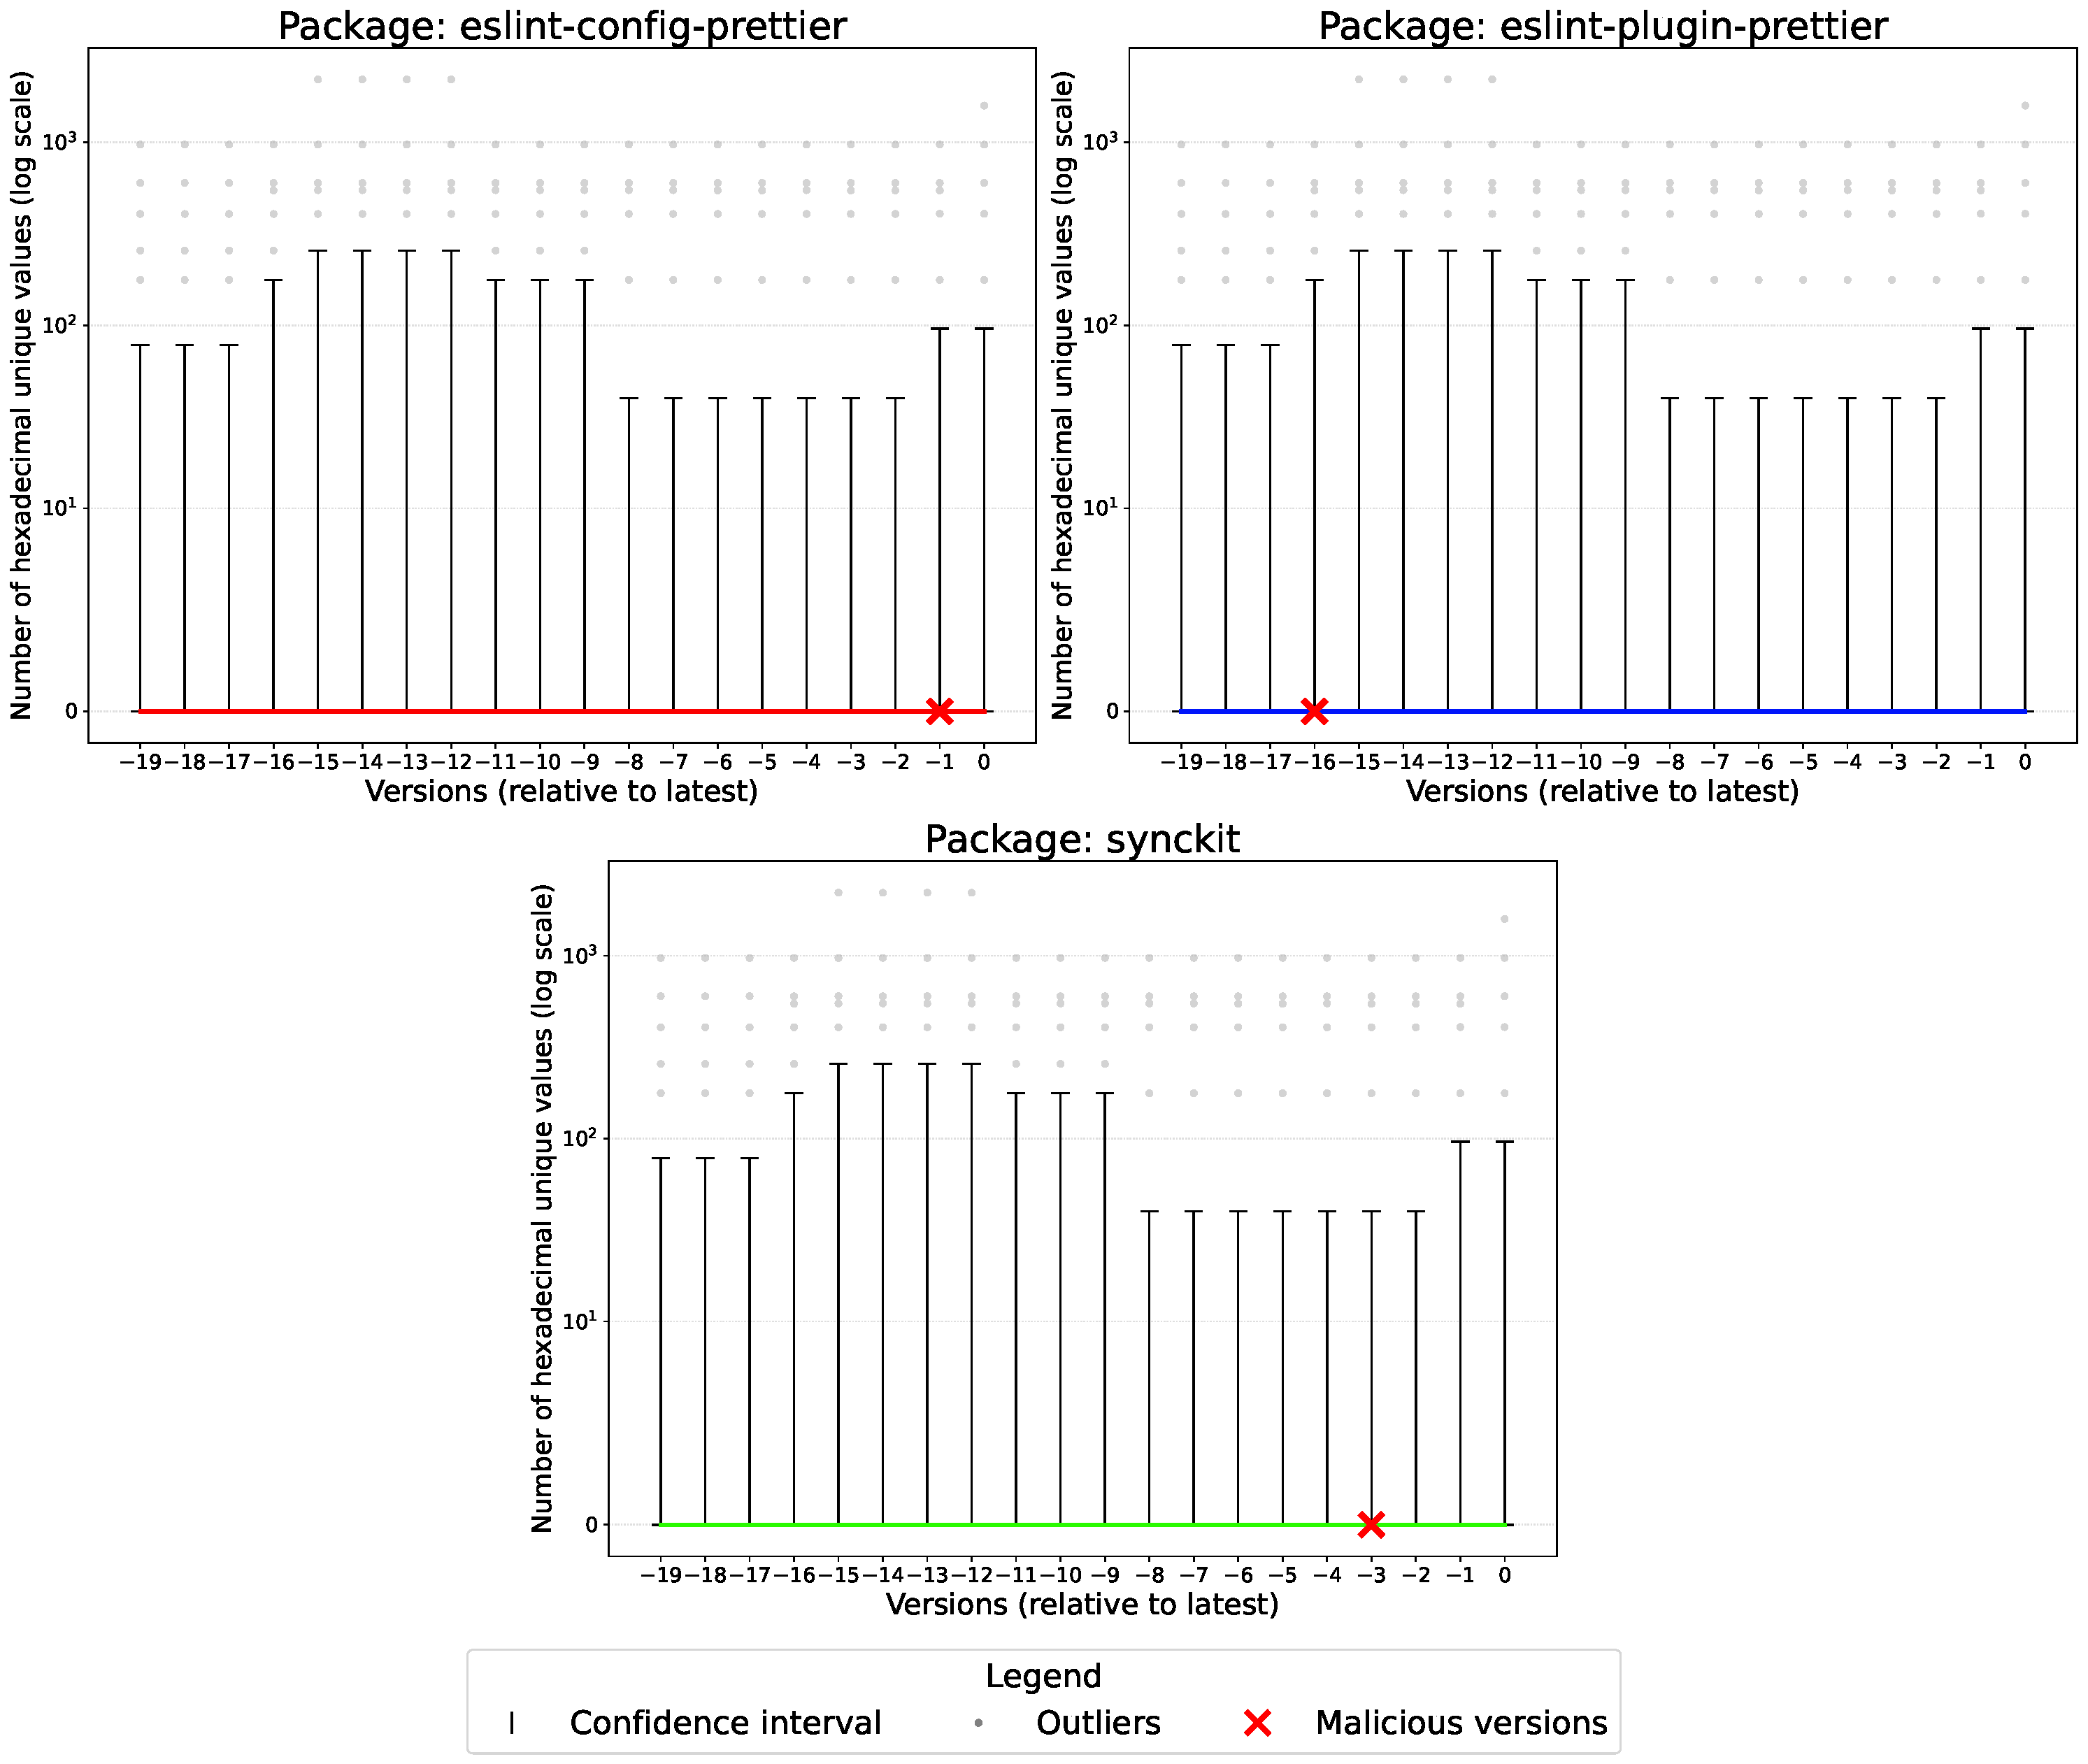
\includegraphics[width=\textwidth]{metrics/hex/hex_plot2singlesingle_AttackA.pdf}
    \caption{Comparison with Malware Dataset Unique Hexadecimal Values Metric for Attack A.}
    \label{fig:fig2HexAttackA}
\end{figure}

In attack A (\cref{sec:attackA}), the attacker did not introduce any new hexadecimal values. 
Therefore, the metric remained unchanged compared to previous versions, as shown in \cref{fig:fig2HexAttackA}.
Consequently, this metric is not indicative for detecting this specific attack.


\subsection*{Attack B: Crypto attack}
\label{sec:analysisHexAttackB}

\begin{figure}[htbp]
    \centering
    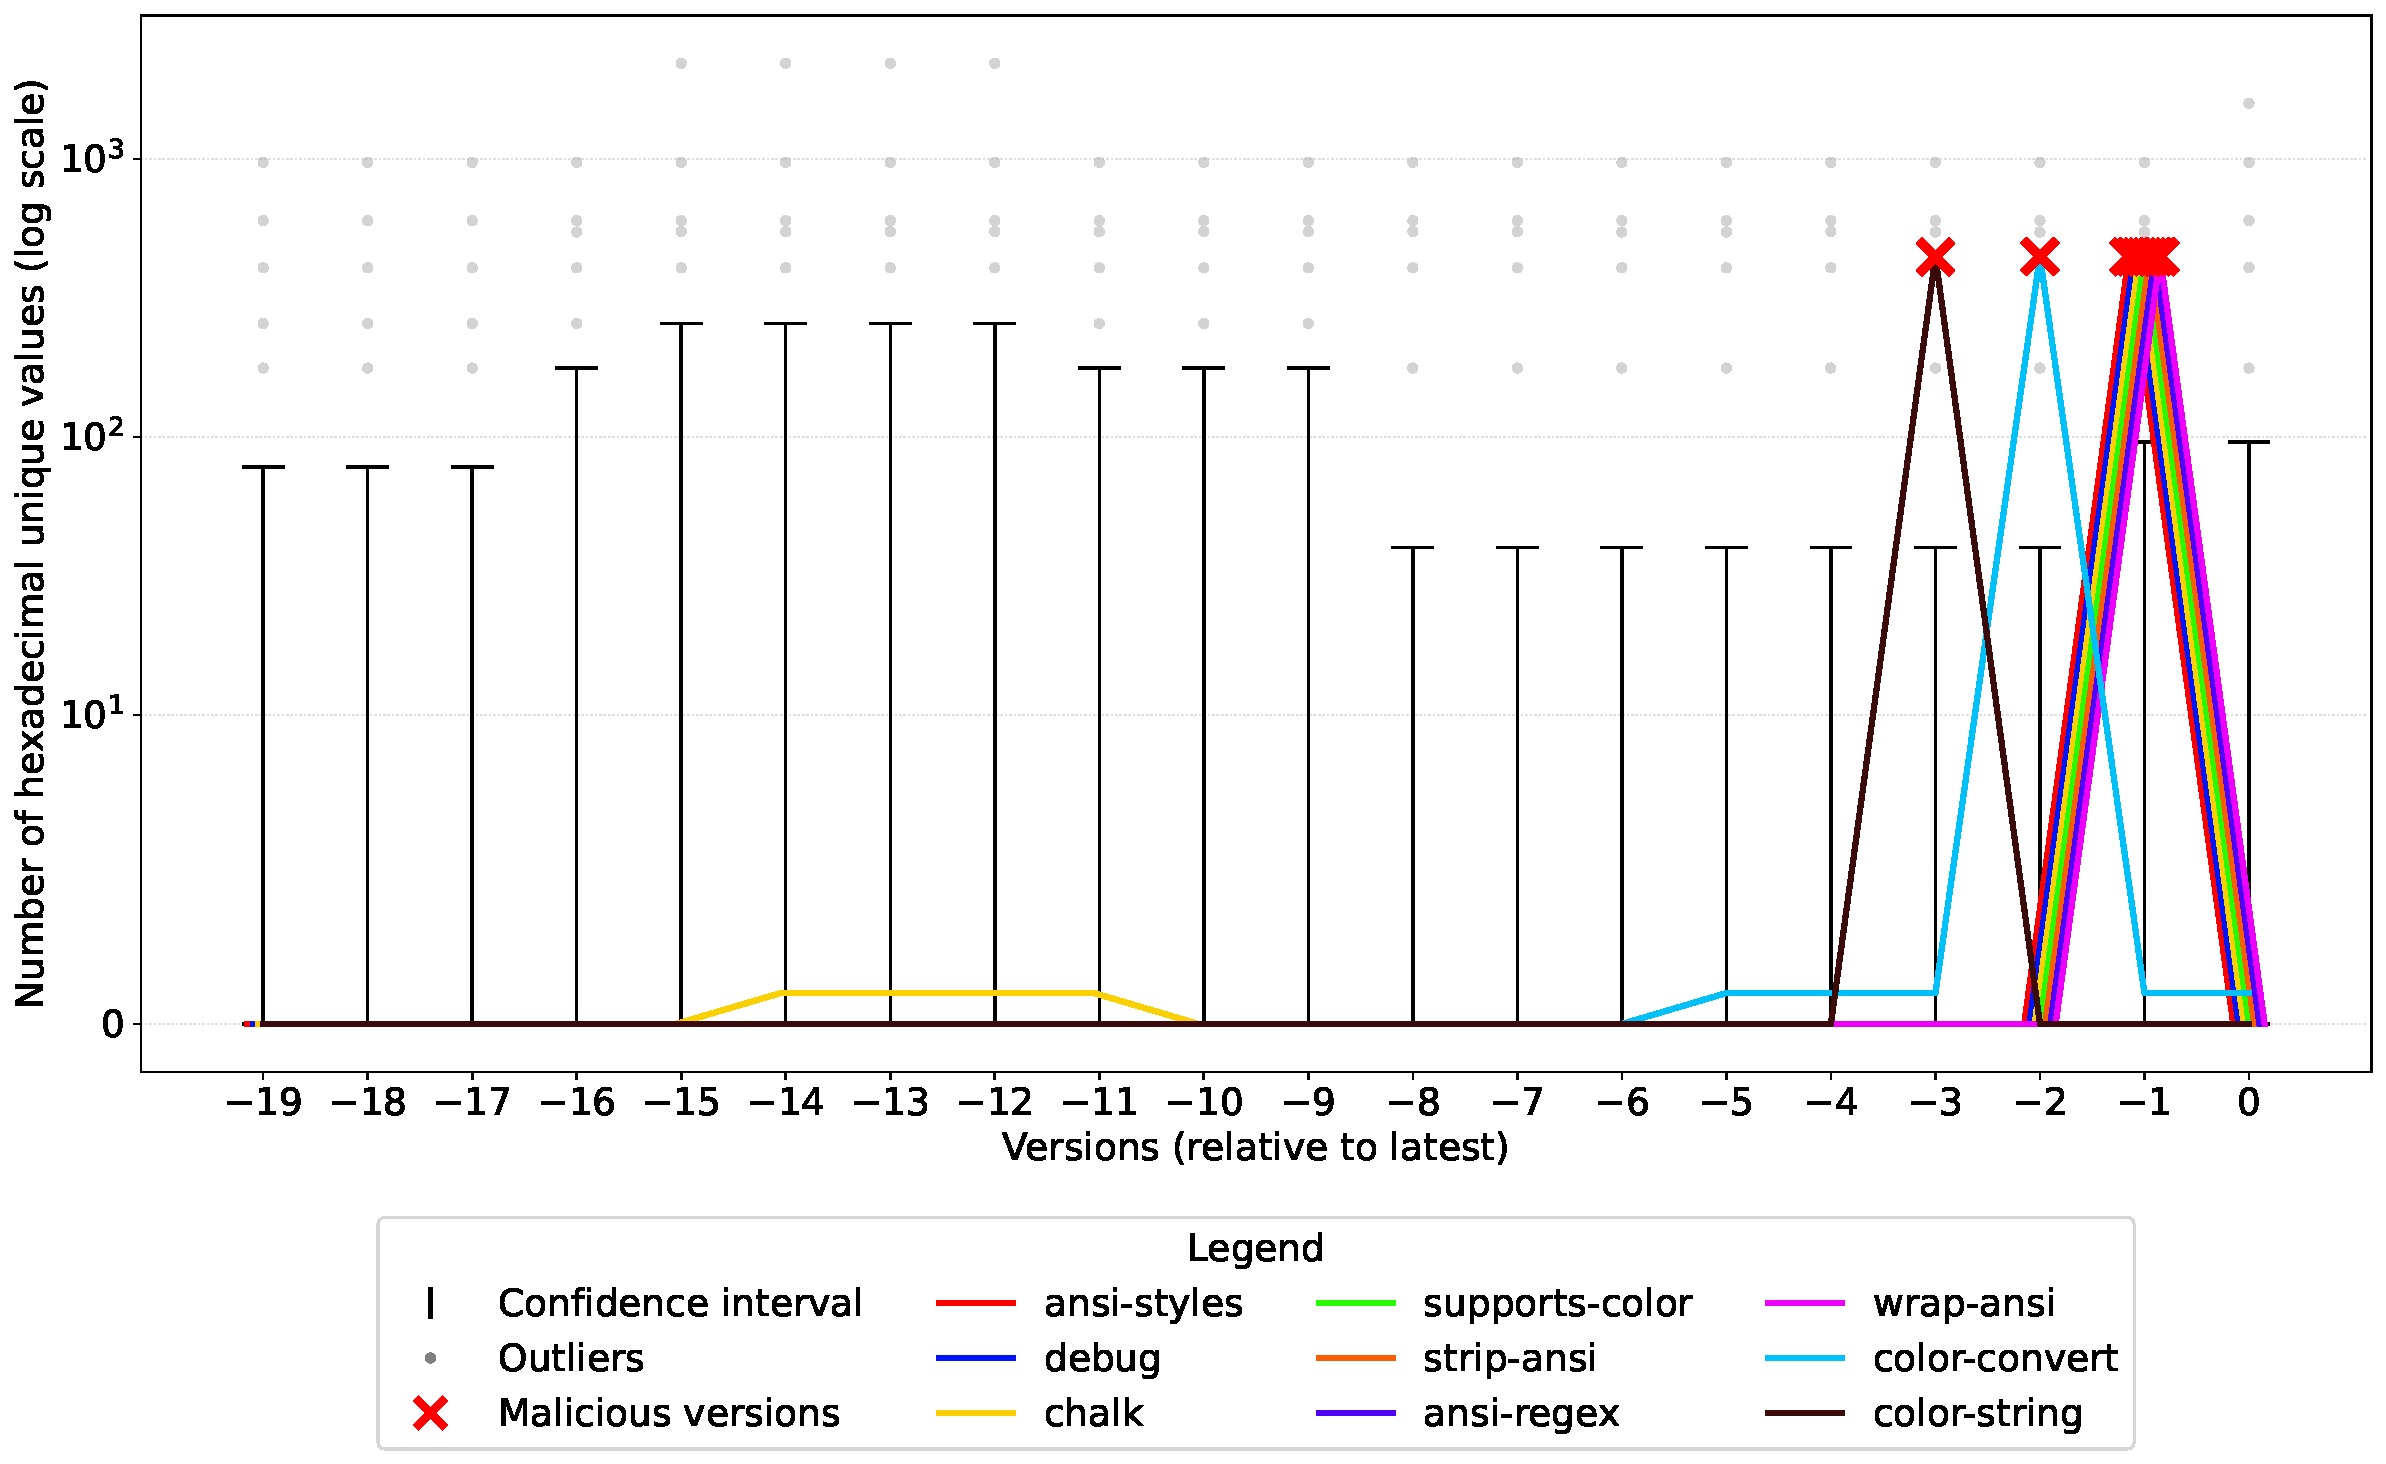
\includegraphics[width=\textwidth]{metrics/hex/hex_plot2single_AttackB.pdf}
    \caption{Comparison with Malware Dataset Unique Hexadecimal Values Metric for Attack B.}
    \label{fig:fig2HexAttackB}
\end{figure}

In attack B (\cref{sec:attackB}), the attacker introduced an obfuscated line 
of code into an existing file, increasing the number of unique hexadecimal values to 455.
As shown in \cref{fig:fig2HexAttackB}, 
this value positions the malicious versions of the packages among the outlier values. 
Therefore, the metric is effective for detecting this specific attack.


\subsection*{Attack C: Shai-Hulud 1.0}
\label{sec:analysisHexAttackC}

\begin{figure}[htbp]
    \centering
    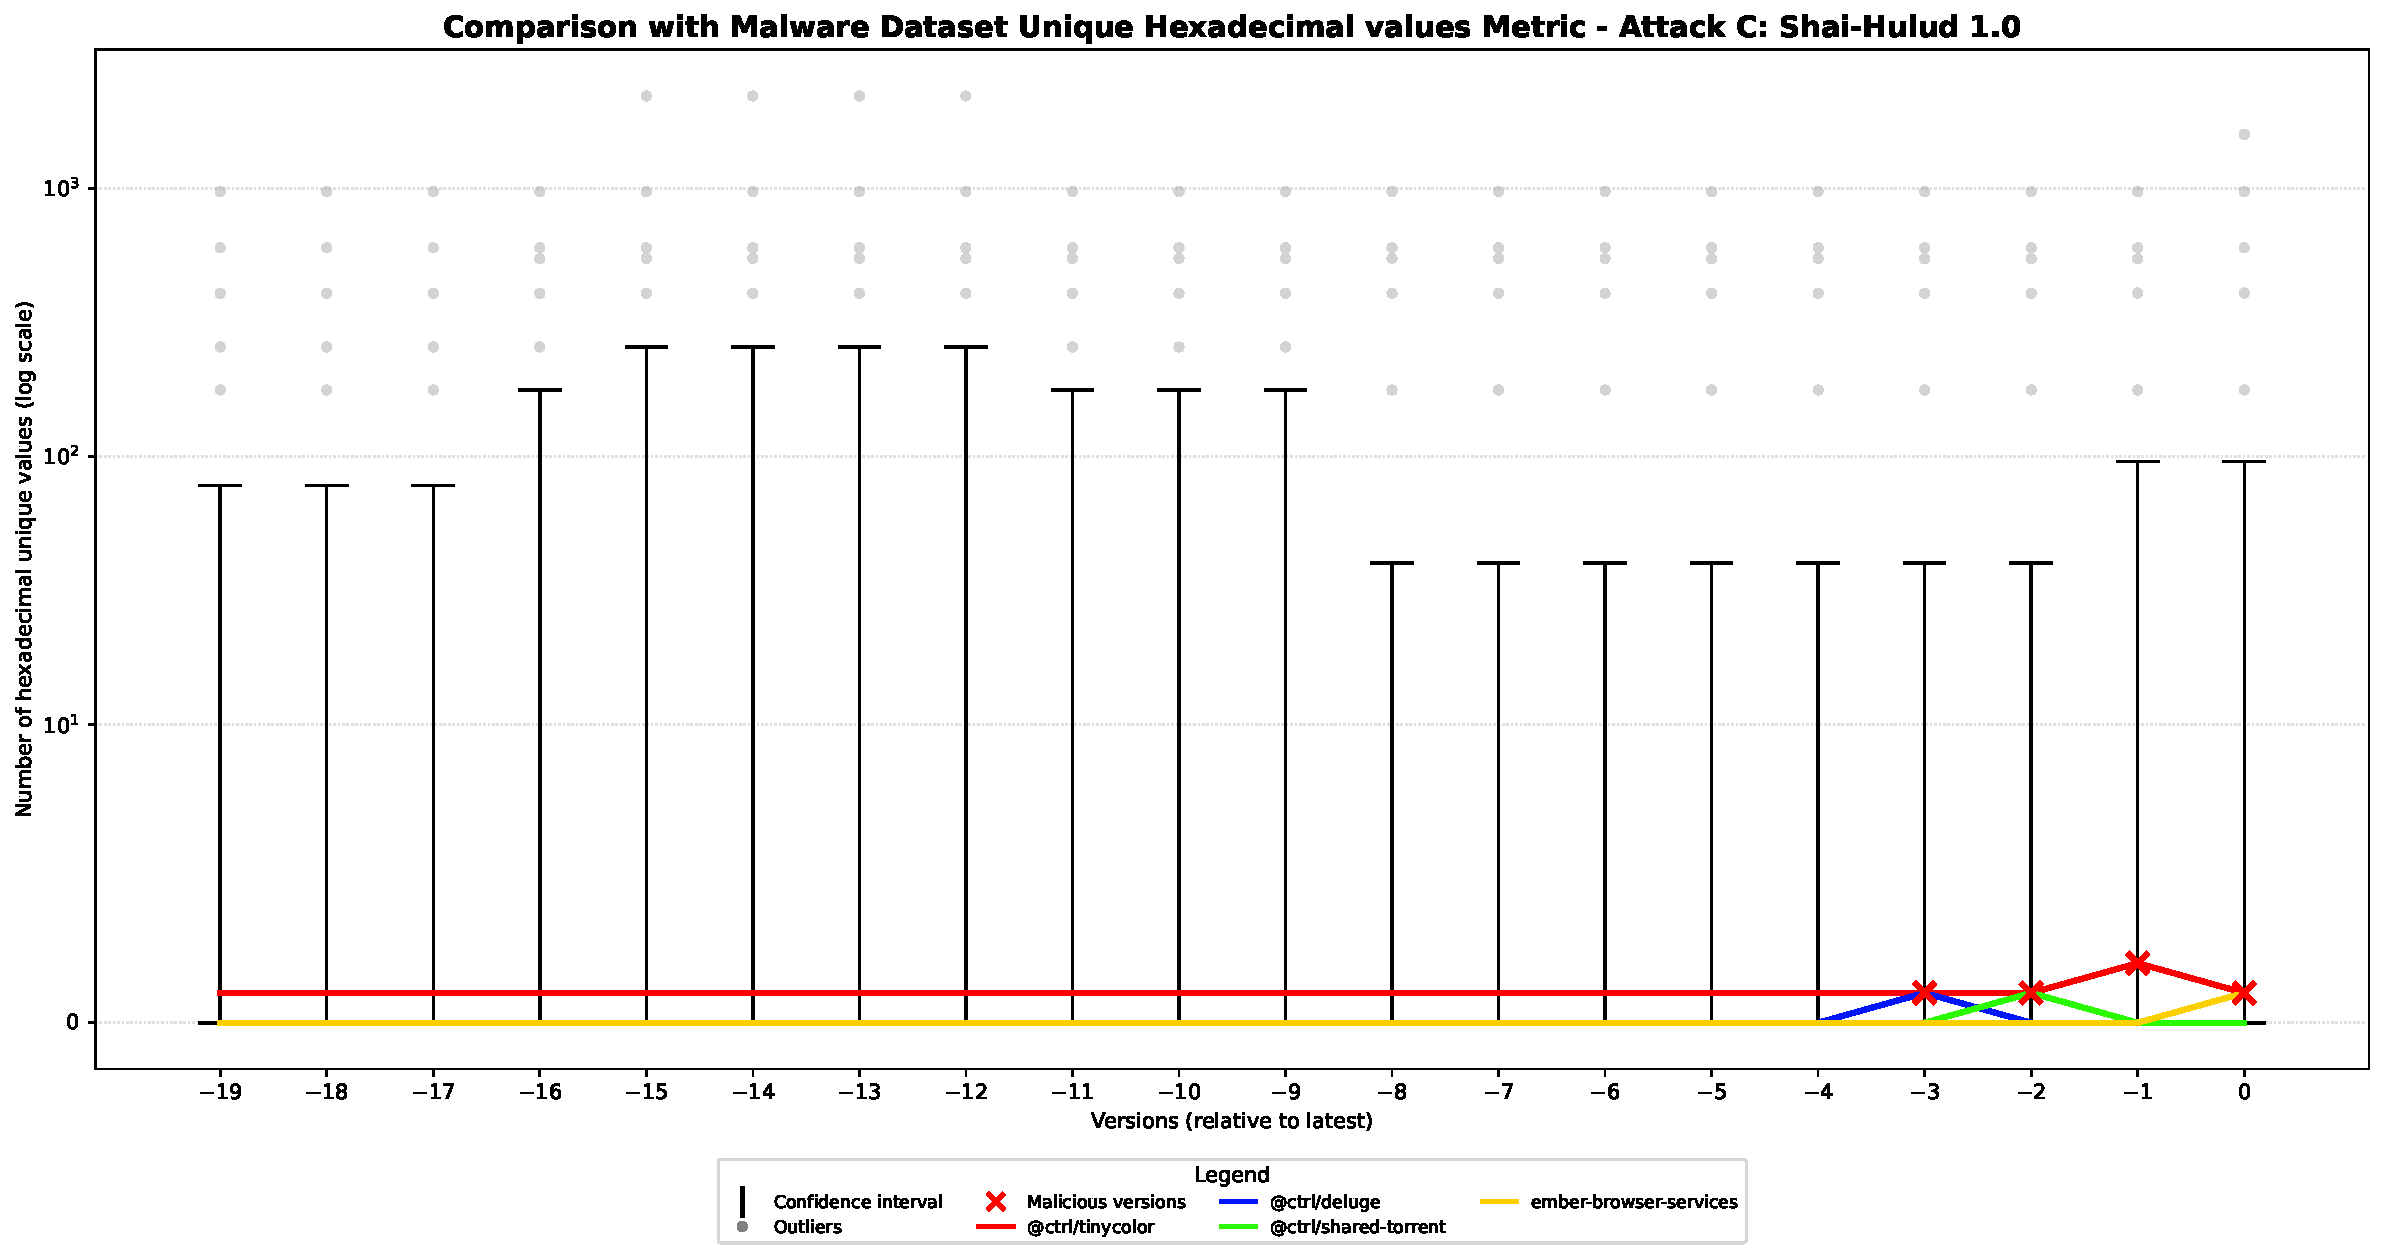
\includegraphics[width=\textwidth]{metrics/hex/hex_plot2single_AttackC.pdf}
    \caption{Comparison with Malware Dataset Unique Hexadecimal Values Metric for Attack C.}
    \label{fig:fig2HexAttackC}
\end{figure}

In attack C (\cref{sec:attackC}), the attacker introduced a malicious clear-text file 
containing only one unique hexadecimal value.
As shown in \cref{fig:fig2HexAttackC}, this marginal increase is insufficient to position the malicious versions 
of the packages outside the confidence intervals.
Consequently, the metric is not indicative for detecting this specific attack, 
as the compromised versions remain indistinguishable from legitimate ones.

\subsection*{Attack D: Shai-Hulud 2.0}
\label{sec:analysisHexAttackD}

\begin{figure}[htbp]
    \centering
    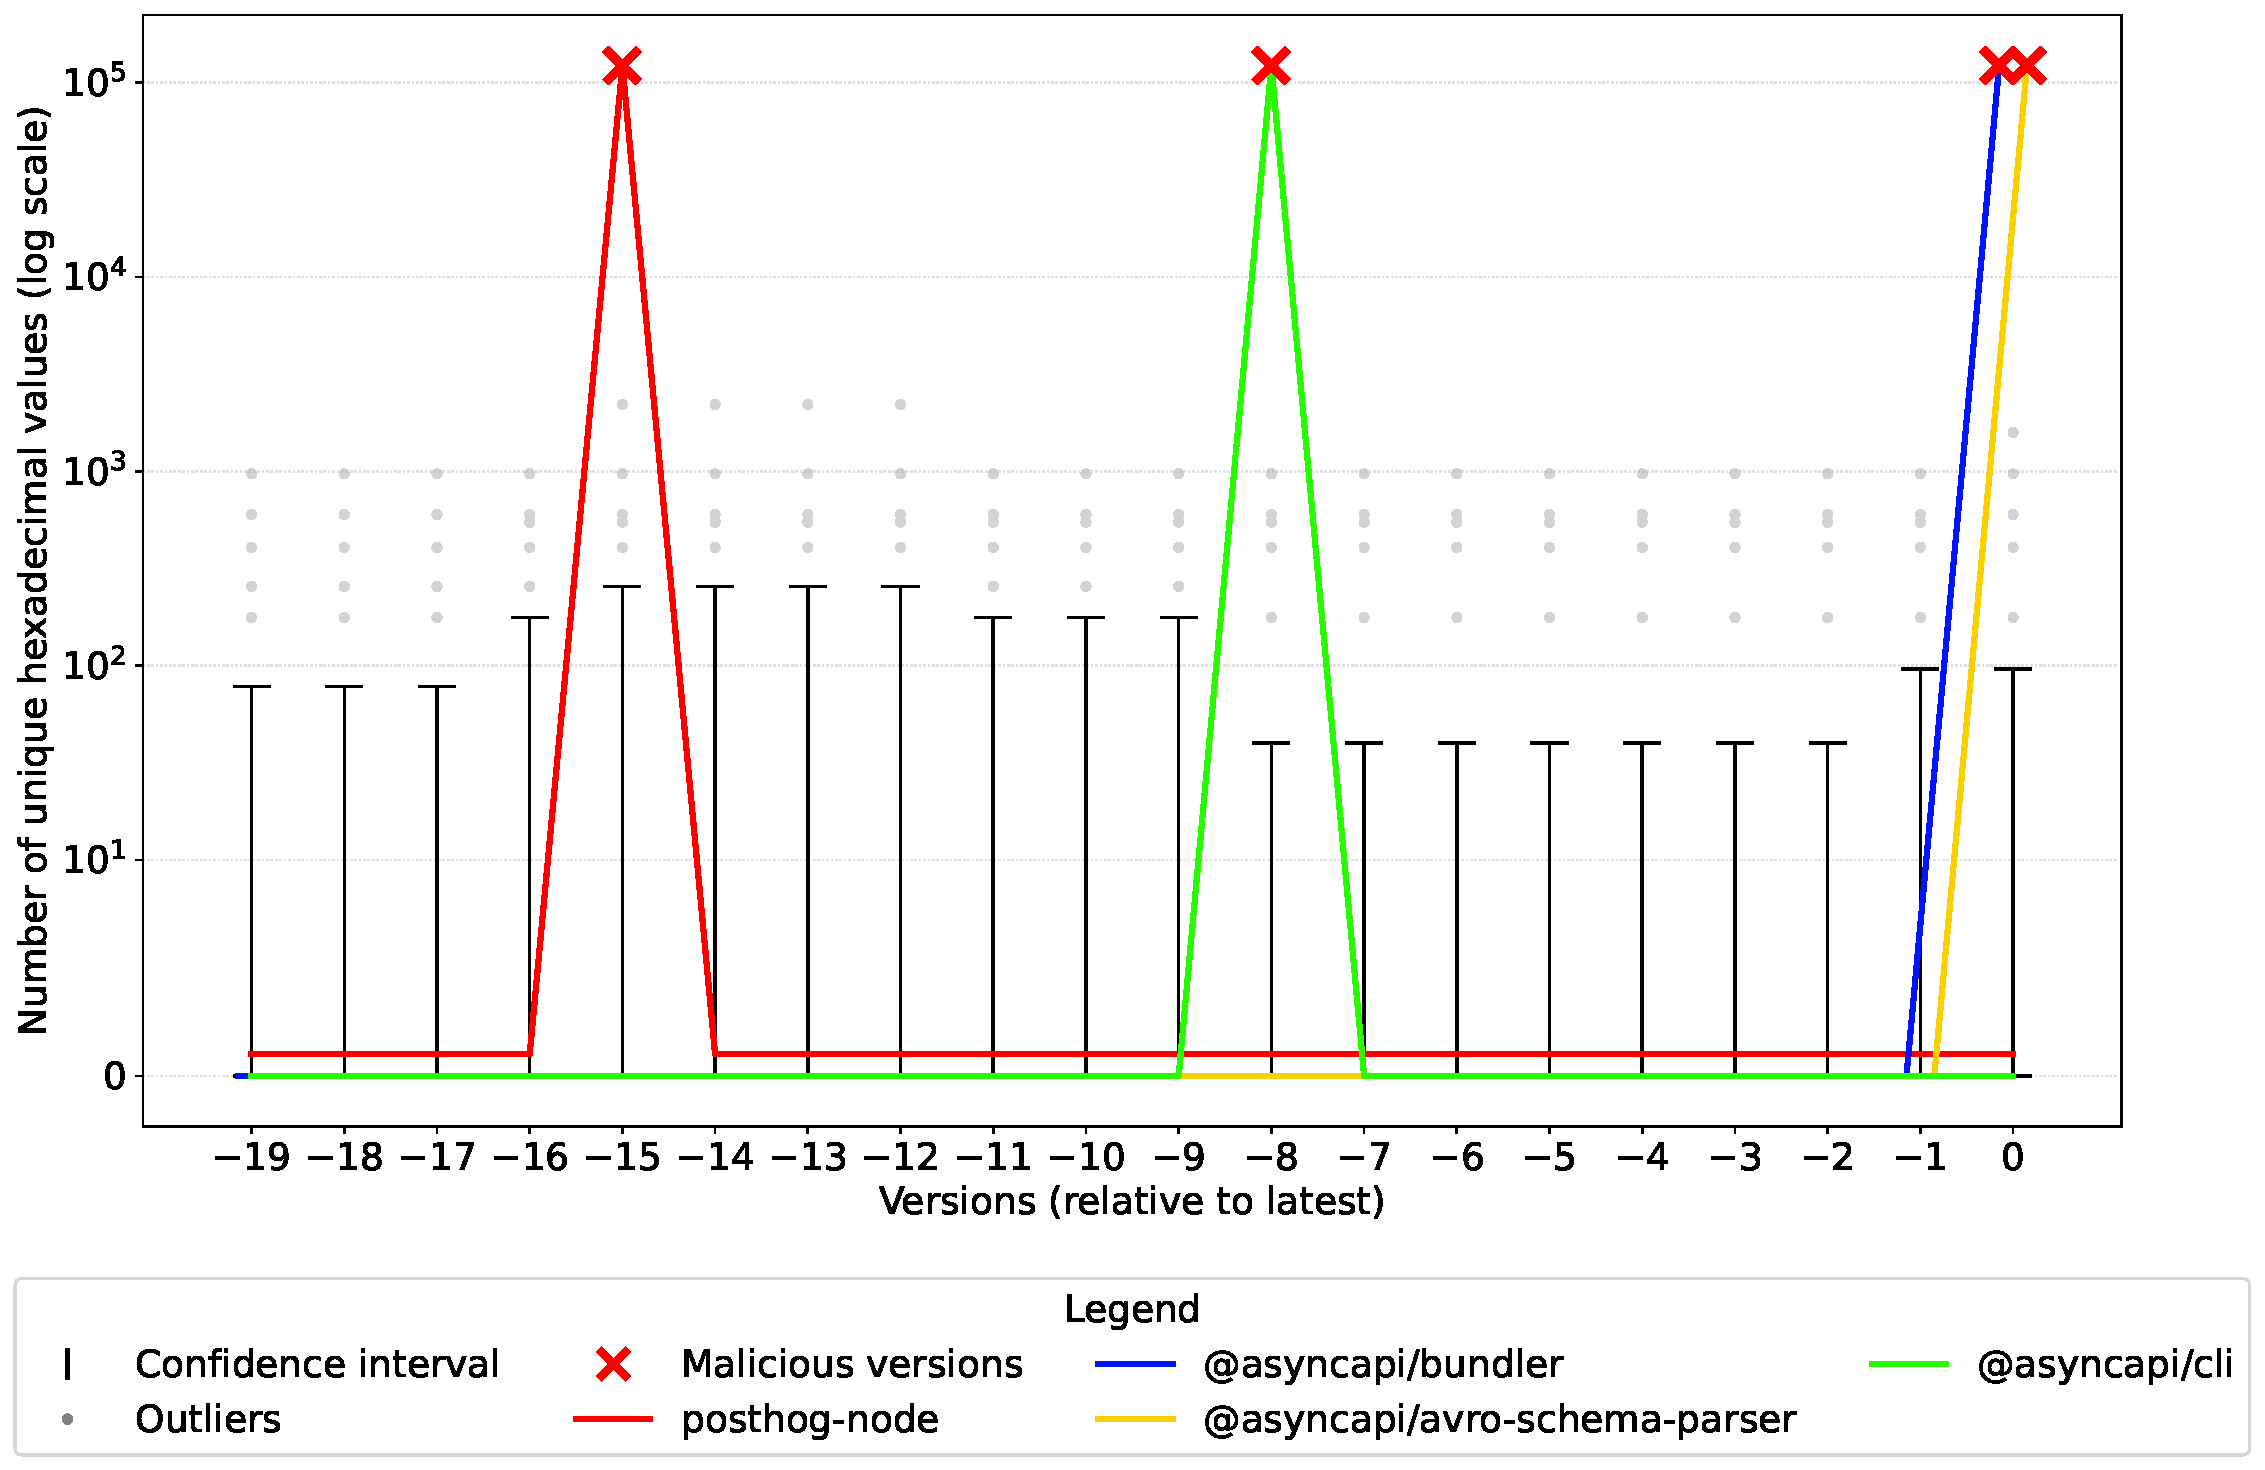
\includegraphics[width=\textwidth]{metrics/hex/hex_plot2single_AttackD.pdf}
    \caption{Comparison with Malware Dataset Unique Hexadecimal Values Metric for Attack D.}
    \label{fig:fig2HexAttackD}
\end{figure}

Finally, in attack D (\cref{sec:attackD}), the attacker introduces an obfuscated malicious file.
As shown in \cref{fig:fig2HexAttackD}, the packages 
with the compromised version have a number of unique hexadecimal values that skyrockets to 122,535, 
far exceeding the maximum outlier values.
Therefore, the metric is effective for detecting this attack.

\subsection*{Summary of Comparison with Malware Dataset}
\label{sec:analysisHexSummaryComparisonMalware}

In summary, the metric is efficient in detecting the attack B (Crypto attack \cref{sec:analysisHexAttackB}) 
and the attack D (\texttt{Shai-Hulud}~2.0 \cref{sec:analysisHexAttackD})
because, in both cases, the malicious versions have a number of unique hexadecimal values that 
qualify as outlier values.

Instead, the metric is not indicative for detecting the attack A (Malicious Windows DLL \cref{sec:analysisHexAttackA}) 
and the attack C (\texttt{Shai-Hulud}~1.0 \cref{sec:analysisHexAttackC}) because, in both cases, 
the malicious versions have a number of unique hexadecimal values that position them within the confidence intervals,
rendering them indistinguishable from legitimate versions.